\chapter{Steve Safety and Limitations} \label{ch:limits}

This chapter discusses the safety guarantees enforced in individual stages
and the pipeline as whole. It will also expand upon the limitations
briefly mentioned in the tutorial from Chapter \ref{ch:tutorial}.

\section{Pipeline Guarantees and Constraints} \label{guide:pipeline_checking}

Steve makes guarantees about the logical correctness and safety of pipeline 
composition using a constraints system. These guarantees are enforced by ensuring each Steve pipeline has two  properties: \textit{progress} and \textit{requirement satisfaction}. Any 
pipeline which does not have these properties is ill-formed. 
Pipelines that cannot ensure these properties risk crashes or undefined behavior.

\subsection{Pipeline to Graph Conversion} \label{guide:pipeline_graph}

These properties are checked by first converting a Steve pipeline into a directed graph, known as a \emph{transition graph}. Each property thus becomes a graph evaluation algorithm on the pipeline graph. 

Let the set of nodes $N$ represent stages in the pipeline: decoders, flow tables, flow entries, event handlers, egress processing, and termination.
Flow entries and inserted flow entries are treated as independent nodes because they are separate branches in pipeline logic.
Added flows cannot violate pipeline properties either, regardless of when they get added.
For each flow entry within a flow table or that would be inserted into a table, let there be a directed edge from the flow table to the flow entry.

For every \texttt{decode}, \texttt{goto}, and \texttt{raise} action found in a stage 
(or flow entry within a table), let there be a directed edge from the stage 
to the destination specified by the action. 
This edge is added even if the action is encapsulated by a conditional statement 
because its impossible to determine during compile time whether or not that edge 
is reachable during runtime.

Let there be a node in $e \in N$ which represents egress processing. For each stage which is not guaranteed to execute a stage transition, let there be an edge from that stage to $e$. Let there be a node $t \in N$ which represents termination. There exists an edge from $e$ to $t$. For any \texttt{drop} action found within a stage, let there be an edge from that stage to $t$. 

Every pipeline graph must have exactly one root node (the starting decoder) and exactly one sink (termination).
If there exists a node where there is no path from the source to that node, it is
considered disconnected from the graph and ignored.

\subsection{Progress} \label{guide:progress}

The \textit{progress} property says that a packet always moves to a later stage in a pipeline and can never move, or risk moving, to a previously visited stage.
This guarantees termination when processing a packet.
Progress is the fundamental nature of the pipeline abstraction. 

A Steve program is well-formed if and only if the graph representation of the pipeline is a directed acyclic graph (DAG). This property can be easily confirmed using topological sorting.

\textit{Proof.} By definition of a DAG and the transition graph, it is obvious that all execution paths end in termination. Note that while loops and function calls may actually result in non-termination.

%First of all, table nodes are assigned a hidden, unique, incremented integer identifier in the order with which they are declared. For example, the first table declared in a Steve program is given the integer identifier 0, the second table declare is given the identifier 1, and so on. Conventionally, tables are expected to be declared in the order with which they are expected to occur in a pipeline.
%
%The \textit{table identifiers} rule says that at no point in the pipeline can a packet reach a target table if it has already visited a table stage whose integer identifier is higher than or equal to that of the target table. In other words, a packet can only go forward through tables, never backwards. This is compliant with the OpenFlow specification for tables \cite{openflow_spec}. Because of this table identifiers rule, it is impossible for any number of table stages to form a cycle with each other.
%
%\textit{Proof.} A cycle can only be formed if the next table has either been visited, or is contained within a path to a table that has been visited. This can only happen if the next table has an identifier less than or equal to that of the current largest identifier visited. This property is enforced by the way tables are numbered. Since the table identifiers rule prevents a packet from being sent to these tables, it is thus impossible to form a cycle.

\subsection{Requirements Satisfaction} \label{guide:requirements}

\textit{Requirement Satisfaction} checks that a field is accessed on after it has been extracted. This prevents accidental access of fields that have not been discovered or that do not exist. For example, consider the pipeline graph in Figure \ref{fig:bad_graph} which demonstrates an ill-formed pipeline where a field is required but not extracted.

\begin{figure}[ht]
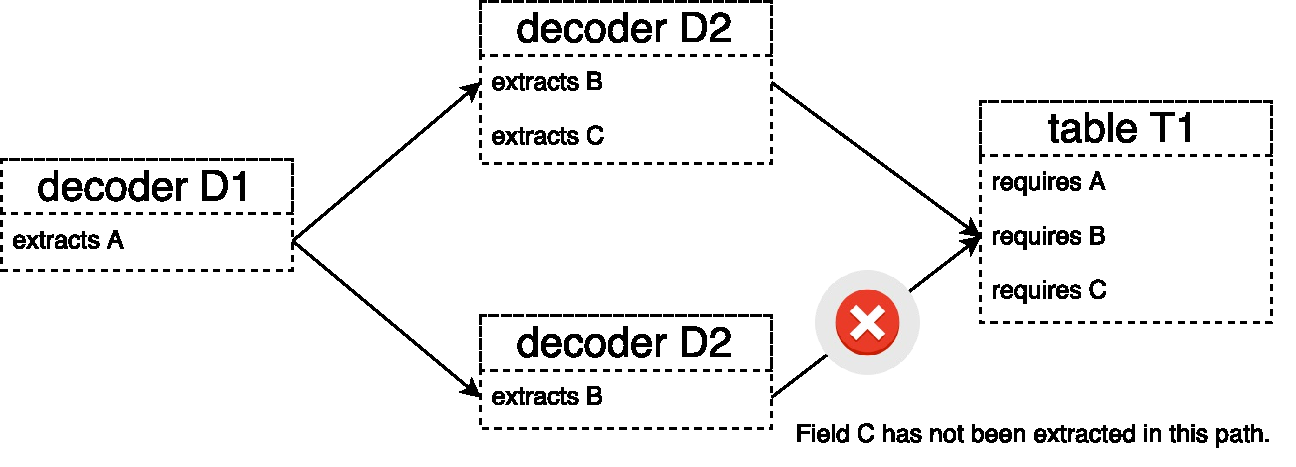
\includegraphics[width=0.85\textwidth]{bad_graph}
\caption{An ill-formed pipeline. Table \texttt{T1} requires fields A, B, and C. However, in the path from \texttt{D1} to \texttt{D3} to \texttt{T1}, field C has not been extracted.}
\label{fig:bad_graph}
\end{figure}

The Steve compiler enforces this
property rather than asking the Steve programmer to check for it.
It avoids runtime checks and reduces the opportunity for programmer error.
To check this property, 
every node in a pipeline graph is associated with a set of \textit{productions} and \textit{requirements}.

A \textit{production} is a field that has been extracted or created by the node's respective stage. Currently only decoding stages are capable of have productions because they are the only ones which can extract fields. If a field were pushed (i.e. created) onto the packet, that would also constitute a production (Steve does not currently support this action).

A \emph{requirement} is a field which must be extracted before reaching a node on
this graph. An event handler's requirements are listed in its
\texttt{requires} specifier. A table's requirements are given by its
key fields, and it may also have a \texttt{requires} specifier.

Let $G$ be the transition graph representing the Steve pipeline.
Let $P$ be the set of all paths from the root node (representing the starting decoder) to a node $n \in G$. 
For a path $p \in P$, let $S$ be the union of all productions of nodes in $p$. 
For $p$ to \emph{satisfy} the requirements of $n$, 
all requirements of $n$ must be a subset of $S$.
If any $p \in P$ does not satisfy the requirements of $n$, then the program
is ill-formed. If all $n \in G$ have their requirements
satisfied, then the program is well-formed, otherwise it is ill-formed.

\textit{Theorem.} Accessing a field can not happen before it has been extracted.

\textit{Proof.} 
Within a decoder, a field may only be accessed after an extract declaration. Within a flow entry, a field may only be accessed if it appears in the table's key's or \texttt{requires} specifier. Within an event handler, a field may only be accessed if it appears within the \texttt{requires} clause. In order to prove that these accesses are valid, it must be shown that field access can only happen if a node has its requirements satisfied.

With a proof by contradiction, assume that field access happened within a node whose requirements were not satisfied, therefore the field has not been extracted. By definition of requirement satisfaction, the pipeline is ill-formed. Therefore, field access could not happen.

%The objective is to prevent field access on fields that have not been extracted. Field access can only be done in three cases. In case 1, the decoder accesses the field.
%In case 2, a flow entry within a table accesses the field. In case 3, an event
%handler accesses the field.
%
%In case 1, a decoder can only use a field after an extract declaration with
%that field name has been made inside that decoder. This innately prevents field access from happening on
%un-extracted fields within a decoder. Since a decoder can only access fields it has decoded, it also has no requirements that must be satisfied by other nodes.
%
%In case 2, the Steve language semantics prevent a flow entry from using
%fields that are not part of the containing flow table's key fields or
%required fields. If all paths leading to the table satisfy its requirements,
%by definition those fields must have been extracted at least once before
%reaching the table. If this is the case, when the flow entry accesses that
%field, it is guaranteed to have been extracted.
%
%In case 3, the Steve language semantics prevent an event handler from using fields
%that are not listed in the \texttt{requires} specifier. If all paths
%leading to an event handler satisfy its requirements, then by definition, it is guaranteed that field has been extracted at least once.

\subsection{Requirements Checking} \label{guide:dfs_desc}

To confirm that all nodes have their requirements satisfied, the Steve compier uses depth-first traversal with backtracking to evaluate all possible paths in a pipeline graph (see Algorithm \ref{alg:dfs}). 

This algorithm assumes that the graph is confirmed to be a DAG first.
As the algorithm traverses a path in the graph, it accumulates a set of productions at each node. That node's requirements are checked against the accumulating set of productions to confirm the \textit{requirement satisfaction} property holds true. Any node which fails immediately indicates the program is ill-formed and further traversal along that path stops.

%At any point in a given path, if a node's edge is directed toward a previously visited node in the path, e.g. a cycle is found, traversal past that node immediately stops and the program is considered ill-formed. This ensures that the \textit{progress} property is met.

Once the algorithm reaches the end of a path successfully, it backtracks to previous
nodes and explores other paths. When backtracking, the algorithm removes the productions of nodes that were left behind.

\begin{algorithm}[ht]
 \caption{Depth-first traversal with backtracking used to check requirement satisfaction.}
 \label{alg:dfs}
 \begin{algorithmic}
 \State
 \State \textit{Input}: Let \textit{G} be the pipeline transition graph. Let \textit{n} be a node in \textit{G}. Let \textit{p} be a set of productions.
 \State \textit{Output}: Whether or not the current stage violates the progress or requirements satisfaction property. If any property fails, output a compiler error.
 \State

 \Function{DFS}{$G, n, p$}
 	\State n.visited = true
 	\State difference = p $\setminus$ n.productions
 	\State p = p $\cup$ n.productions
 	\If{n.requirements $\subseteq$ p} \Comment{Check for requirement satisfaction.}
 		\For{\textit{all} a \textit{in} G.adjacentNodes(n)}
 			\If{a.visited == false}
 				\State \Call{DFS}{G, a, p}
 			\Else
 				\State \Return ill-formed
 			\EndIf
 		\EndFor
	\Else
 		\State \Return ill-formed
 	\EndIf
 	
	
 	\State n.visited = false \Comment{Reset the visited property so we can come down this node again in a different path.}

 	\State p = p $\setminus$ difference \Comment{Remove the productions of this node from the set of productions when backtracking.}
 \EndFunction
 \end{algorithmic}

\end{algorithm}

\textit{Theorem.} The worst case complexity of this algorithm is $O(n!)$ where $n$ is the number of nodes.

\textit{Complexity Proof.}  Assume a DAG has $n$ nodes. There are at most $n-1$ nodes adjacent to the root node. Each node adjacent to the root has at most $n-2$ nodes adjacent to it. This pattern continues until paths end in a sink. Thus the number of paths can be represented as $(n-1)(n-2)...1$ or $(n-1)!$. Therefore, the performance
is $O(n!)$.

Fortunately, this worst case performance is rarely ever achieved. Only the most dense pipeline graphs, where a node at each level is connected to every other possible node has this kind of performance. Packet processing graphs are typically closer to trees as branches only occur when determining what the next header is. These graphs are generally not very deep either as packets tend to have a very small number of headers.
Additionally, it is acceptable to incur performance penalties at compile time
to ensure safety at runtime.

\textit{Termination Proof.} By definition, a DAG has a finite number of unique paths that can be taken from source to sink, therefore, it must terminate if it takes every unique path exactly once.
%A unique path, by definition, is an ordered sequence of nodes that is distinct from all other paths.
%Let $V$ be the set of all nodes in the graph $G$.
%For a graph traversal algorithm to visit the same path more than once.
%
%Consider the base case.
%Let $s$ be the root node for the graph. By Steve semantics, there may only be one start node. Let $A$ be the set of nodes adjacent to $s$. If the edge from $s$ to any $a \in A$ has been traversed, it is not possible to move from $s$ to $a$, therefore, the same path cannot be traversed twice from $s$.
%
%Now considering the recursive case, let $v$ be any other node in the graph. By definition of a DAG, $v$ must be the root of some subgraph $G'$ in $G$ that is also a DAG. Let $A'$ be the set of adjacent nodes to $v$. For each node $a' \in A'$, the $DFS(G',v, p)$ traverses the edge from $v$ to $a'$ exactly once. If this algorithm does not terminate, then the algorithm must be able to traverse from $v$ to any node $a' \in A'$ more than once, which is not the case. Note that is is possible to apply the algorithm to $G'$ multiple times, but because there are a fixed number of paths from $s$ to a sink in $G$, it is executed a fixed number of times.

\section{Why Objects of Layout Type can not Exist.} \label{guide:no_dst}

It was mentioned in an earlier chapter than objects of layout type may not exist.
This is necessary for two reasons.
First, Steve does not currently support creating new packets or pushing new headers. 
It can only processing existing ones. 
Objects of layout type are not strictly necessary without this ability.
Second, there are a number of concerns related to construction objects whose
types are dynamically sized.

Allocating objects of dynamically-sized types (DST) on the stack produce a number of concerns which have not been solved.
The only language which actually supports user-defined DSTs, Rust, only allows it under 
very limited circumstance \cite{rust_dst_std}.
Allocating DST objects on the heap is, of course, what dynamic allocation was made for, but
it is expensive and does not help when reinterpreting existing packet memory.
Allocating a single DST object on the stack is not actually a difficult thing to achieve. 
It is done by allocating memory by pushing the stack pointer forward using the intrinsic
\texttt{alloca}. 
Now consider what happens when this DST object appears at the end of a class/record
type. For example:

\begin{codepage}
\begin{lstlisting}
struct Ipv4 {
	version : uint(4);
	ihl : uint(4);
	// ...
	// options has dynamically-sized type predicated on ihl.
	options : DST(ihl); 
}

var x : Ipv4 = ...;
\end{lstlisting}
\end{codepage}

The \texttt{options} member has a length predicated on the value
of another member in the object. In order to produce an object of type \texttt{Ipv4},
first the memory for the object must be allocated. Then the value of \texttt{ihl}
has to be evaluated. Then the memory for that object has to be \emph{extended}
using \texttt{alloca}. This is possible because \texttt{options} is the last member in the class. Though tricky, this is still possible and roughly what the Rust does.
However, now consider what happens when the DST member is \emph{not} at the end
of the class, but rather the middle. For example:

\begin{codepage}
\begin{lstlisting}
struct FooClass {
	x : int;
	y : DST(x);
	z : int;
}
\end{lstlisting}
\end{codepage}

Only \texttt{x} can be allocated at first. The value of \texttt{x} has to be evaluated
and only then could \texttt{y} and \texttt{z} be allocated. It becomes impossible
for the compiler to reason about the actual position of \texttt{z} in memory. This 
makes member access on \texttt{z} an extremely expensive runtime computation.
Then consider that an object of type \texttt{FooClass} may also appear in
another class, making it even more difficult to manage.

Because of these unclear issues, Steve has forgone allowing objects of DSTs.
By extension, because layouts have to have DST fields, objects of layout type
are also not allowed.


\section{Decoder Anatomy} \label{decoder_anatomy}

This section discusses the ``anatomy'' of a decoder.
Specifically, it will describe the formalism of \textit{(offset, length)} generation by the compiler, what unexpected circumstances
may arise while decoding, and a special kind of extraction known
as a rebinding.

\subsection{Determining the Location and Length of Extracted Fields}

An extract declaration produces an extraction by executing a set of instructions on a packet which saves the extraction's \textit{location} and \textit{length} to the context's binding environment. Information gathered from the field name and layout rule is used to calculate these two values. These instructions are completely opaque to the user and are automatically generated by the compiler. The formalism for this code generation is described below.

First, let the field name have the form \texttt{E1.E2} where \texttt{E1} is the \textit{container layout} and \texttt{E2} is the \textit{contained field}.

\begin{enumerate}
\item The length of the extracted field is calculated by a function $len(E2)$. The result of $len(E2)$ is the \textit{size} of an object of $E2$'s type.

\item  Let $precede(E1, E2)$ be a function that returns the sequence of all field declarations preceding \texttt{E2} in \texttt{E1}. 

\item The function used to calculate the \textit{relative offset} of $E2$ is given as $rel(E1, E2)$ and is defined as:

\begin{enumerate}

\item If \texttt{E1} identifies a layout, then $rel(E1, E2) = \sum_{x \in precede(E1,E2)}{} len(x)$.

\item If \texttt{E1} is a field name, then let \texttt{E1} have the form \texttt{E1'}.\texttt{E2'}.

Then $rel(E1, E2)=rel(E1', E2') + \sum_{x \in precede(E2',E2)}{} len(x)$

\end{enumerate}

\item If $rel(E1, E2)$ results in a number greater than the length of the field, then the packet is malformed and dropped.

\item Given a field name of the form \texttt{E1.E2} and the current view index (see \ref{guide:decoder_view}), $i$, the \textit{absolute offset} of the field being extracted is this $abs(E1, E2) = i + rel(E1, E2)$.
If the result of $abs(E1, E2)$ is greater than the length of the packet, then the packet is malformed and dropped.

\item The location of an extracted field is its absolute offset, that is, the number of bytes it is away from the beginning of the packet. The pair stored by the binding environment is $(abs(E1, E2), len(E2))$.

\end{enumerate}

Consider the following example. Two layouts, \texttt{L} and \texttt{N}, and a decoder, \texttt{D}, are provided.

\begin{minip}
\begin{lstlisting}
layout L {
	a : uint;
	b : uint;
	c : N;
}
layout N {
	d : uint(8);
	f : uint(16);
}
decoder D(L) {
	extract L.a;
	extract L.c.f;
}
\end{lstlisting}
\end{minip}

\texttt{L} has three fields: \texttt{a}, \texttt{b}, and \texttt{c}.  \texttt{N} has two fields: \texttt{d} and \texttt{f}. Field \texttt{L.c} has layout type \texttt{N} and is thus a nested layout. \texttt{D} decodes \texttt{L} and extracts \texttt{L.a} and \texttt{L.c.f}.

The first extract declaration is \texttt{extract L.a}. The type of \texttt{a} is \texttt{uint} (32 bit unsigned integer by default). The result of $len(a)$ is 32 bits or 4 bytes. The relative offset of \texttt{a} in \texttt{L} is the sum of the lengths of all field declaration which precede it. In this case, no fields precede it, thus its relative offset is 0.

The second extract declaration is \texttt{extract L.c.f}. This is the case of the nested layout. The value of $len(f)$ is 16 bits or 2 bytes. The relative offset of \texttt{f} is the sum of the length of all field declaration which precede it in \texttt{N} (8 bits or 1 byte), plus the relative offset of \texttt{c} in \texttt{L} (64 bits or 8 bytes). Thus, the relative offset for \texttt{L.c.f} is $64+8=72$ bits or 9 bytes.

Assuming an arbitrary example where the beginning of the current view for \texttt{D} is 112 bits past the beginning of the packet, the \textit{absolute offset} for \texttt{L.a} would be 112 bits. The absolute offset for \texttt{L.c.f} would be $112+72=184$ bits or 23 bytes.

\subsection{Extracting the Same Field More Than Once}

A common misunderstand happens when an extract appears within a loop.
A decoder is only ever looking at one header of a packet at once. Using an extract declaration with the same field name more than once in the same decoder will result in the same instance of that field being extracted multiple times, which is completely redundant. Though legal, this should be avoided in most cases. For example: 

\begin{minip}
\begin{lstlisting}
while (x < 5)
	extract L1.f1;
\end{lstlisting}
\end{minip}


%The extractions which \texttt{N1} can refer to are a subset of the extractions \texttt{N2} can refer to. The aliased name naturally can refer to extractions which are from a different kind of field than the original name. To demonstrate this, the following revision is made to the prior example:
%
%\begin{minip}
%\begin{lstlisting}
%decoder D1(L1) {
%	extract L1.a;
%	if (L1.a == 0)
%		goto T1;
%	
%	decode d2;
%}
%
%decoder D2(L2) {
%	extract L2.c as L1.a;
%	// Valid usage of L2.c.
%	var i : uint(16) = L2.c;
%	// Valid usage of L1.a to refer to the same extraction.
%	var j = uint(16) = L1.a;
%
%	set L2.c = 1;
%	goto T1;
%}
%
%// Key field L1.a will refer to the last extraction of L1.a.
%// If D1 sends the packet to T1, then it will be the L1.a field.
%// 
%// If D2 sends the packet to T1, then L1.a shall refer to an
%// extraction of L2.c instead.
%exact_table T1(L1.a) {
%	{ 0 } -> { drop; }
%	{ 1 } -> { flood; }
%}
%\end{lstlisting}
%\end{minip}
%
%This example presents decoders \texttt{D1} and \texttt{D2}. If a packet is sent directly to table \texttt{T1} from decoder \texttt{D1}, the value of the last extraction of \texttt{L1.a} will be \texttt{0} (based on the \texttt{if} condition). In this scenario, the packet is dropped. 
%
%However, if the packet is sent from decoder \texttt{D2}, the field \texttt{L2.c} has been aliased as \texttt{L1.a}. The field \texttt{L2.c} has its value set to \texttt{1}. \texttt{L1.a} refers to the same value as L2.c because of the rebinding, therefore, the value of L1.a is also \texttt{1}.
%When the packet is matched against \texttt{T1}'s flow entries, the packet shall be flooded.
%
%Supposing table \texttt{T1} from the prior example were replaced with the following version of \texttt{T1}, then the \texttt{goto T1} action in decoder \texttt{D1} would actually produce a compiler error for violating requirements satisfaction (see \ref{guide:requirements}). 
%
%\begin{minip}
%\begin{lstlisting}
%exact_table T1(L2.c) { ... }
%\end{lstlisting}
%\end{minip}
%
%This version of \texttt{T1} uses \texttt{L2.c} as a key field. However, \texttt{L1.a} is not the same field as \texttt{L2.c} and has not been aliased as such.

